% Versión 3.0 (19/01/2022)
% Daniel (danieeelxy@gmail.com)


% Preámbulo

\documentclass[a4paper, 9pt, openany, oneside]{memoir}


% Ruta de archivos, instalación de paquetes y ruta de imágenes

\makeatletter
\def\input@path{{/path/}}
\makeatother

\usepackage{geometry}
\usepackage{xcolor}
\usepackage[mathrm=sym]{unicode-math}
\usepackage{fontspec}
\usepackage{fancyhdr}
\usepackage{titlesec}
\usepackage{graphicx}
\usepackage[spanish]{babel}
\usepackage{embrac}
\usepackage{contour}
\usepackage[normalem]{ulem}

\usepackage{bm}
\usepackage{amsmath}
\usepackage{amsthm, amsfonts}
\usepackage{centernot}
\usepackage{mathtools}
\usepackage{mathrsfs}
\usepackage{cancel}
\usepackage{siunitx}
\usepackage{mhchem}

\usepackage{caption}
\usepackage{multicol}
\usepackage{tabu}
\usepackage{array}
\usepackage{hyperref}
\usepackage[nosectionbib]{apacite}
\usepackage{enumitem}
\usepackage{calc}
\usepackage{afterpage}
\usepackage{tcolorbox}
\tcbuselibrary{skins, listings, breakable, theorems}

\usepackage{tikz}
% \usetikzlibrary{matrix, decorations.pathreplacing, hobby, arrows, shapes, decorations.markings, calc, decorations, decorations.pathmorphing}
% \usepackage{tkz-euclide}
\usepackage{pgfplots}
% \pgfplotsset{compat=newest}
\usepackage{circuitikz}
\usepackage{pst-electricfield}

\graphicspath{{./img/}}


% Definición de comandos

% Colores misceláneos

\definecolor{egyptianblue}{RGB}{16,62,166}
\definecolor{firebrickred}{RGB}{178,34,34}
\definecolor{carbon}{RGB}{25,25,25}
\definecolor{astroblue}{RGB}{22,101,175}
\definecolor{darkgreen}{RGB}{0,152,70}
\definecolor{darktealblue}{RGB}{0,66,121}


% Paleta de colores pastel

\definecolor{pastelpink}{RGB}{237,211,216}
\definecolor{pastelred}{RGB}{255,177,177}
\definecolor{pastelorange}{RGB}{255,208,168}
\definecolor{pastelyellow}{RGB}{255,243,170}
\definecolor{pastelgreen}{RGB}{126,252,204}
\definecolor{pastelcyan}{RGB}{183,239,255}
\definecolor{pastelblue}{RGB}{179,224,255}


% Colores semánticos

\colorlet{foot}{gray!50}
\colorlet{titlecounter}{gray!75}
\colorlet{cover}{darktealblue}
\colorlet{block}{egyptianblue!70}
\colorlet{slab}{firebrickred}
% Tamaño de letra gigante

\makeatletter
\renewcommand\HUGE{\@setfontsize\Huge{38}{47}} 
\makeatother

\makeatletter
\newcommand\HUGe{\@setfontsize\Huge{30}{35}} 
\makeatother


% Fuente genérica (títulos, portada, figuras, tablas, etc.)

\newcommand{\setgenfont}[1]{
	\newfontfamily\genfamily{#1}
	\newenvironment{genericfont}{\genfamily}{\par}
	\DeclareTextFontCommand{\textgen}{\genfamily}
	}

\setgenfont{Lato}


% Fuente nombre

\newcommand{\setsignaturefont}[1]{
	\newfontfamily\signaturefamily{#1}
	\newenvironment{signaturefont}{\signaturefamily}{\par}
	\DeclareTextFontCommand{\textsignature}{\signaturefamily}
	}

\setsignaturefont{Lato}


% Fuente principal y matemática

\setmainfont[SmallCapsFont={Latin Modern Roman Caps}]{Latin Modern Roman}
\setmathfont{Latin Modern Math}
% Márgenes

\geometry{hmargin=3cm, vmargin=2cm}


% Encabezados y pies de página

\newcommand{\titulo}[1]{
	\hypersetup{pdftitle={Apuntes de #1}}
	\lfoot{\small\genfamily\itshape\color{foot}#1}
	}
\newcommand{\autor}[1]{
	\hypersetup{pdfauthor={#1}}
	\rfoot{\small\genfamily\color{foot}#1}
	}

\cfoot{\small\genfamily\color{foot}\thepage}

\renewcommand{\chaptermark}[1]{\markboth{#1}{#1}}
\chead{\small\genfamily\color{foot}\leftmark}

\rhead{}
\lhead{}

\renewcommand{\headrulewidth}{0pt}
\renewcommand{\footrulewidth}{0pt}

\pagestyle{fancy}


% Encabezado para el índice

\fancypagestyle{index}{
	\chead{\small\genfamily\color{foot}Índice}
	}
% Contadores de enumeración

\setcounter{secnumdepth}{3}
\setcounter{tocdepth}{3}
\renewcommand{\thechapter}{\Roman{chapter}}
\renewcommand{\thesection}{\arabic{section}}


% Espacio entre enumeración y nombre

\newcommand{\marginsecnumber}[1]{\makebox[0pt][r]{#1\hspace{6pt}}}


% Formato de títulos

\titleformat{\chapter}[display]
	{\genfamily\mdseries}
	{\centering\genfamily\HUGe\textcolor{titlecounter}{\thechapter}}
	{0cm}
	{\centering\Huge\genfamily\bfseries\MakeUppercase}

\titleformat{\section}[hang]
	{\Large\genfamily\bfseries}
	{\marginsecnumber{\textcolor{titlecounter}{\thesection}}}
	{0cm}
	{\Large\genfamily\bfseries}

\titleformat{\subsection}[hang]
	{\large\genfamily\bfseries}
	{\marginsecnumber{\textcolor{titlecounter}{\thesubsection}}}
	{0cm}
	{\large\genfamily\bfseries}

\titleformat{\subsubsection}[hang]
	{\normalsize\genfamily\bfseries}
	{\marginsecnumber{\textcolor{titlecounter}{\thesubsubsection}}}
	{0cm}
	{\normalsize\genfamily\bfseries\itshape}
% Distancia entre párrafos e indentación

\setlength{\parskip}{0.25cm}
\setlength{\parindent}{1cm}


% Definición de contadores

\renewcommand{\thetable}{\arabic{chapter}.\arabic{table}}
\renewcommand{\thefigure}{\arabic{chapter}.\arabic{figure}}
\renewcommand{\theequation}{\arabic{chapter}.\arabic{equation}}


% Etiquetas de figuras y tablas

\DeclareCaptionFont{gf}{\genfamily}
\captionsetup[figure]{font={small}, labelfont={bf, gf}, name={Figura}}
\captionsetup[table]{font={small}, labelfont={bf, gf}, name={Tabla}}
\captionsetup{width=0.8\textwidth}


% Configuración de listas

\renewcommand{\labelenumi}{\bfseries\genfamily\textup{\arabic{enumi})}}
\renewcommand{\labelenumii}{\bfseries\genfamily\textup{\alph{enumii})}}
\renewcommand{\labelenumiii}{\bfseries\genfamily\textup{\roman{enumiii})}}
\renewcommand{\labelitemi}{\bullet}
\renewcommand{\labelitemii}{---}

\setlist{itemsep=0.1cm, leftmargin=0.5cm, parsep=0.1cm}


% Configuración de unidades

\sisetup{output-decimal-marker={,}}
\sisetup{separate-uncertainty=true}
\sisetup{per-mode=reciprocal}
\sisetup{bracket-unit-denominator=true}
\sisetup{detect-weight=true}


% Subrayado

\renewcommand{\ULdepth}{0.06cm}
\contourlength{0.02cm}
\contournumber{64}

\newcommand{\subr}[2][black]{{\color{#1}\uline{\phantom{#2}}}\llap{\contour{white}{#2}}}
% Definición de la portada

\newcommand{\cover}[3]{
	\setcounter{page}{0}
	\thispagestyle{empty}
	\pagecolor{cover}
	\color{white}
	\begin{center}
	
\includegraphics[width=2cm]{saturn_white.eps}
	\end{center}
	\begin{center}
	\genfamily
	\vspace*{\fill}
	\HUGE\uppercase{\textbf{\textit{#1}}}\\
	\vspace*{\fill}
	\Huge\textsignature{#2}\\
	\vspace*{0.25cm}
	{\normalsize#3}
	\end{center}
	\newpage
	\pagecolor{white}
	\color{black}
	}
% Tabla de contenidos

\renewcommand{\printtoctitle}[1]{\centering\Huge\genfamily\bfseries\MakeUppercase#1}
\renewcommand{\aftertoctitle}{\thispagestyle{fancy}\afterchaptertitle}
\renewcommand*{\cftchapterpagefont}{\bfseries\genfamily}
\renewcommand*{\cftsectionpagefont}{\small\genfamily}
\renewcommand*{\cftsubsectionpagefont}{\small\genfamily}
\renewcommand*{\cftchapterfont}{\bfseries\genfamily}
\renewcommand*{\cftsectionfont}{\small\genfamily}
\renewcommand*{\cftsubsectionfont}{\small\genfamily}
\renewcommand{\cftsectionaftersnum}{.}
\addto\captionsspanish{\renewcommand{\contentsname}{Índice}}
\setlength{\cftsectionindent}{0.5cm}
\setlength{\cftsubsectionindent}{1cm}
\setlength{\cftchapternumwidth}{0.5cm}
\setlength{\cftsectionnumwidth}{0.5cm}
\setlength{\cftsubsectionnumwidth}{0.5cm}


% Comando inicial de portada y tabla de contenidos

\newcommand{\start}[3]{%
	\cover{#1}{#2}{#3}%
	\tableofcontents%
	\thispagestyle{index}
	}
% Fijar estilo de referencias

\bibliographystyle{apacite}


% Fijar estilo español

\AtBeginDocument{
	\renewcommand\bibname{Bibliografía}
	\renewcommand{\BCBT}{}
	\renewcommand{\BCBL}{}
	\renewcommand{\BOthers}[1]{et al.\hbox{}}
	\renewcommand{\BOthersPeriod}[1]{y otros.\hbox{}}
	\renewcommand{\BAnd}{y}
	\renewcommand{\BBAA}{y}
	\renewcommand{\BBAB}{y}
	}


% Espacio entre referencias de la bibliografía

\setlength{\bibitemsep}{0.25cm}


% Comando inicial de bibliografía

\newcommand{\finish}[1]{
	\bibliography{#1}
	\thispagestyle{fancy}
	}

% Definición de parte real e imaginaria

\AtBeginDocument{\renewcommand{\Re}{\mathfrak{Re}}}
\AtBeginDocument{\renewcommand{\Im}{\mathfrak{Im}}}


% Definición de símbolos de conjuntos

\AtBeginDocument{\renewcommand{\varnothing}{\diameter}}
\AtBeginDocument{\renewcommand{\setminus}{\smallsetminus}}
\newcommand{\normal}{\unlhd}
\newcommand{\parts}[1]{\mathcal{P}\parn*{#1}}
\newcommand{\Matrix}[2]{\mathcal{M}_{#1}\parn*{#2}}
\newcommand{\GL}[1]{\mathrm{GL}\parn*{#1}}
\newcommand{\SL}[1]{\mathrm{SL}\parn*{#1}}
\newcommand{\Ort}[1]{\mathrm{O}\parn*{#1}}
\newcommand{\SO}[1]{\mathrm{SO}\parn*{#1}}


% Vectores, matrices y símbolos diferenciales

\newcommand{\ve}[1]{\symbfup{#1}}
\newcommand{\vi}[1]{\symbfit{#1}}
\newcommand{\un}[1]{\hat{\symbfup{#1}}}
\newcommand{\dif}{\mathrm{d}}
\newcommand{\Dif}{\mathrm{D}}
\def\difbar{{\mathchar'26\mkern-12mu d}}
\newcommand{\tp}{{\mathsf{T}}}


% Símbolo QED

\renewcommand{\qedsymbol}{\(\blockfull\)}


% Flechas y cancelación

\renewcommand{\implies}{\Rightarrow}
\renewcommand{\iff}{\Leftrightarrow}
\newcommand{\inyto}{\hookrightarrow}
\newcommand{\epito}{\twoheadrightarrow}

\let\cancelorigcolor\CancelColor
\newcommand{\xcancelto}[3][]{
	\ifblank{#1}{}{
		\renewcommand{\CancelColor}{#1}
		}
	\cancelto{#2}{#3}
	}


% Comandos de fuentes

\newcommand{\bb}[1]{\mathbb{#1}}
\renewcommand{\cal}[1]{\mathcal{#1}}
\newcommand{\scr}[1]{\mathscr{#1}}

\DeclareSymbolFontAlphabet{\amsmathbb}{AMSb}
\newcommand{\A}{\amsmathbb{A}}
\newcommand{\B}{\amsmathbb{B}}
\newcommand{\C}{\amsmathbb{C}}
\newcommand{\D}{\amsmathbb{D}}
\newcommand{\E}{\amsmathbb{E}}
\newcommand{\F}{\amsmathbb{F}}
\newcommand{\G}{\amsmathbb{G}}
\renewcommand{\H}{\amsmathbb{H}}
\newcommand{\I}{\amsmathbb{I}}
\newcommand{\J}{\amsmathbb{J}}
\newcommand{\K}{\amsmathbb{K}}
\renewcommand{\L}{\amsmathbb{L}}
\newcommand{\M}{\amsmathbb{M}}
\newcommand{\N}{\amsmathbb{N}}
\renewcommand{\O}{\amsmathbb{O}}
\renewcommand{\P}{\amsmathbb{P}}
\newcommand{\Q}{\amsmathbb{Q}}
\newcommand{\R}{\amsmathbb{R}}
\renewcommand{\S}{\amsmathbb{S}}
\newcommand{\T}{\amsmathbb{T}}
\newcommand{\U}{\amsmathbb{U}}
\newcommand{\V}{\amsmathbb{V}}
\newcommand{\W}{\amsmathbb{W}}
\newcommand{\X}{\amsmathbb{X}}
\newcommand{\Y}{\amsmathbb{Y}}
\newcommand{\Z}{\amsmathbb{Z}}


% Símbolos físicos

\newcommand{\lagrangian}{\mscrL}
\newcommand{\hamiltonian}{\mscrH}
\newcommand{\routhian}{\mscrR}
\newcommand{\photon}{\upgamma}
\newcommand{\electron}{\mathrm{e}}
\newcommand{\proton}{\mathrm{p}}
\newcommand{\neutron}{\mathrm{n}}
\newcommand{\eneutrino}{\upnu_{\mathrm{e}}}
\newcommand{\antieneutrino}{\bar{\upnu}_{\mathrm{e}}}
\newcommand{\avogadro}{N_{\text{A}}}
\newcommand{\boltzmann}{k_{\text{B}}}
\newcommand{\NA}{\avogadro}
\newcommand{\kB}{\boltzmann}


% Delimitadores

\newcommand{\tq}{\,\middle|\,}

\DeclarePairedDelimiter\ceil{\lceil}{\rceil}
\DeclarePairedDelimiter\floor{\lfloor}{\rfloor}
\DeclarePairedDelimiter\parenthesis{(}{)}
\DeclarePairedDelimiter\brackets{[}{]}
\DeclarePairedDelimiter\rbrackets{[}{)}
\DeclarePairedDelimiter\lbrackets{(}{]}
\DeclarePairedDelimiter\braces{\{}{\}}
\DeclarePairedDelimiter\verts{|}{|}
\DeclarePairedDelimiter\vverts{\|}{\|}
\DeclarePairedDelimiter\angl{\langle}{\rangle}
\DeclarePairedDelimiter\rbar{.}{|}
\DeclarePairedDelimiter\bbrackets{\lBrack}{\rBrack}
\DeclarePairedDelimiter\ket{|}{\rangle}
\DeclarePairedDelimiter\bra{\langle}{|}
\DeclarePairedDelimiterX\braket[2]{\langle}{\rangle}{#1\tq#2}


% Delimitadores (semántico)

\newcommand{\set}{\braces}
\newcommand{\abs}{\verts}
\newcommand{\norm}{\vverts}
\newcommand{\parn}{\parenthesis}
\newcommand{\class}{\brackets}
\newcommand{\open}{\parenthesis}
\newcommand{\closed}{\brackets}
\newcommand{\ropen}{\rbrackets}
\newcommand{\lclosed}{\rbrackets}
\newcommand{\lopen}{\lbrackets}
\newcommand{\rclosed}{\lbrackets}
\newcommand{\eval}{\rbar}
\newcommand{\conm}{\brackets}
\newcommand{\poisson}{\braces}
% Definición de comandos para definir o redefinir operadores

\newcommand{\newoperator}[2]{\DeclareMathOperator{#1}{\mathrm{#2}}}
\newcommand{\renewoperator}[2]{\renewcommand{#1}{\operatorname{\mathrm{#2}}}}


% Definición de operadores

\newoperator{\dom}{dom}
\newoperator{\rec}{rec}
\newoperator{\cod}{cod}
\newoperator{\im}{im}
\newoperator{\interior}{int}
\newoperator{\adh}{adh}
\newoperator{\der}{der}
\newoperator{\fr}{fr}
\newoperator{\arccsc}{arccsc}
\newoperator{\arcsec}{arcsec}
\newoperator{\arccot}{arccot}
\newoperator{\sech}{sech}
\newoperator{\csch}{csch}
\newoperator{\arcsinh}{arcsinh}
\newoperator{\arccosh}{arccosh}
\newoperator{\arctanh}{arctanh}
\newoperator{\arccsch}{arccsch}
\newoperator{\arcsech}{arcsech}
\newoperator{\arccoth}{arccoth}
\newoperator{\id}{id}
\newoperator{\sgn}{sgn}
\newoperator{\gr}{gr}
\newoperator{\diag}{diag}
\newoperator{\ran}{ran}
\newoperator{\Log}{Log}
\newoperator{\charac}{char}
\newoperator{\rot}{rot}
\newoperator{\grad}{grad}
\newoperator{\Aut}{Aut}
\newoperator{\Ennd}{End}
\newoperator{\Inn}{Inn}
\newoperator{\Outt}{Out}
\newoperator{\ord}{ord}
\newoperator{\mcm}{mcm}
\newoperator{\mcd}{mcd}
\newoperator{\Res}{Res}
\newoperator{\dvg}{div}
\newoperator{\Var}{\V ar}
\newoperator{\Cov}{\C ov}
\newoperator{\ecm}{ecm}
\newoperator{\Ei}{Ei}
\newoperator{\intsi}{si}
\newoperator{\li}{li}
\newoperator{\Si}{Si}
\newoperator{\Ci}{Ci}
\newoperator{\erf}{erf}
\newoperator{\erfc}{erfc}


% Redefinición de operadores

\renewoperator{\sin}{sin}
\renewoperator{\cos}{cos}
\renewoperator{\tan}{tan}
\renewoperator{\csc}{csc}
\renewoperator{\sec}{sec}
\renewoperator{\cot}{cot}
\renewoperator{\arcsin}{arcsin}
\renewoperator{\arccos}{arccos}
\renewoperator{\arctan}{arctan}
\renewoperator{\sinh}{sinh}
\renewoperator{\cosh}{cosh}
\renewoperator{\tanh}{tanh}
\renewoperator{\coth}{coth}
\renewoperator{\exp}{exp}
\renewoperator{\ln}{ln}
\renewoperator{\log}{log}
\renewoperator{\arg}{arg}
\renewoperator{\dim}{dim}
\renewoperator{\ker}{ker}
\renewoperator{\det}{det}

% Definición de bloque de color

\newtcolorbox{block}[1]{
	before upper={\parindent0cm},
	parbox=false,
	colback=white,
	colframe=block,
	fonttitle=\color{white}\genfamily\bfseries,
	title={#1},
	arc=1mm,
	arc is angular,
	breakable
	}

\newtcolorbox{slab}[1]{
	empty,
	left=2cm,
	before upper={\parindent0cm},
	parbox=false,
	coltitle=slab,
	fonttitle=\genfamily\bfseries,
	borderline horizontal={0.5mm}{0pt}{pastelred},
	title={#1},
	attach boxed title to top left,
	breakable
	}


% Definición de teoremas y definiciones

\newcounter{theorem}
\renewcommand{\thetheorem}{\arabic{chapter}.\arabic{theorem}}
\newtcbtheorem[auto counter, number within=chapter, number freestyle={\noexpand\arabic{chapter}.\noexpand\arabic{\tcbcounter}}]{theorem}{Teorema}{
	before upper={\parindent0cm},
	parbox=false,
	colback=white,
	colframe=block,
	fonttitle=\color{white}\genfamily\bfseries,
	description font=\itshape,
	arc=1mm,
	arc is angular,
	breakable,
	label separator=*
	}{th}

\newcounter{definition}
\renewcommand{\thedefinition}{\arabic{chapter}.\arabic{theorem}}
\newtcbtheorem[auto counter, number within=chapter, number freestyle={\noexpand\arabic{chapter}.\noexpand\arabic{\tcbcounter}}]{definition}{Definición}{
	empty,
	left=2cm,
	before upper={\parindent0cm},
	parbox=false,
	coltitle=slab,
	fonttitle=\genfamily\bfseries,
	description font=\itshape,
	borderline horizontal={0.5mm}{0pt}{pastelred},
	attach boxed title to top left,
	breakable,
	label separator=*
	}{def}
\input{lib/env/tables}


% Configuración inicial

\autor{Daniel Lobos}
\titulo{Documento de prueba}

\begin{document}

\start{Título de la pixula long very long}{Daniel}{2022}

\chapter{Capítulo}

\thispagestyle{fancy}

\section{Hola}

\[
\A\parn*{B_e\kB}+\sin(\arcsin(y))+p_f+p_\text{libre}\,\mathrm{hola}\,J_{\un{k}}
\]

\textcolor{pastelpink}{Hola \(\A\)}
\textcolor{pastelred}{Hola \(\A\)}
\textcolor{pastelorange}{Hola \(\A\)}
\textcolor{pastelyellow}{Hola \(\A\)}
\textcolor{pastelgreen}{Hola \(\A\)}
\textcolor{pastelcyan}{Hola \(\A\)}
\textcolor{pastelblue}{Hola \(\A\)}

\begin{definition}{Pichula}{def*a}
ooo texto pixula
\end{definition}

\begin{definition*}{Oooooo pixula pixula}%{th*a}
ooo texto pixula
\end{definition*}

\begin{theorem}{}{th*a}
ooo texto pixula
\end{theorem}

\begin{theorem}{Oooooo pixula pixula}{a}
ooo texto pixula
\end{theorem}

\begin{theorem*}{Oooooo pixula pixula}%{th*a}
ooo texto pixula
\end{theorem*}

\begin{block}{Hola}
chao chao chao chao chao chao chao ooo el teorrema \ref{th*th*a} chao chao chao chao chao chao chao chao chao chao chao chao chao chao chao chao chao chao chao chao chao chao chao chao chao chao chao chao chao chao chao chao \subr[egyptianblue]{c google hao chao chao chao chao chao chao python/Que} chao chao chao chao chao chao chao chao chao chao chao chao chao chao chao chao chao chao chao chao chao chao chao chao ch\emph{ao chao chao chao chao chao cha}o chao chao chao chao chao chao chao chao chao chao chao chao chao chao chao chao chao chao chao chao chao chao chao chao chao chao chao chao chao chao chao chao chao chao chao chao chao chao chao chao chao chao chao chao chao chao chao chao chao chao chao chao chao chao chao

\textit{chao chao chao chao chao chao chao chao chao \emph{chao chao chao chao chao chao chao chao chao chao chao chao chao chao chao chao chao chao chao chao chao chao chao} chao
hola hola hola hola hola hola hola hola hola hola hola hola}
\end{block}

\begin{slab}{Chao}
chao chao chao chao chao chao chao chao chao chao chao chao chao chao chao chao chao chao chao chao chao chao chao chao chao chao chao chao chao chao chao chao chao chao chao chao chao chao chao chao chao chao chao chao chao chao chao chao chao chao chao chao chao chao chao chao chao chao chao chao chao chao chao chao chao chao chao chao chao chao chao chao chao chao chao chao chao chao chao chao chao chao chao chao chao chao chao chao chao chao chao chao chao chao chao chao chao chao chao chao chao chao chao chao chao chao chao chao chao chao chao chao chao chao chao chao chao chao chao chao chao chao chao chao chao chao chao chao chao chao chao chao

\[
a^2=b^2+c^2
\]

chao chao chao chao chao chao chao chao chao chao chao chao chao chao chao chao chao chao chao chao chao chao chao chao chao chao chao chao chao chao chao chao chao
hola hola hola hola hola hola hola hola hola hola hola hola
\end{slab}

\chapter{Nombre del primer capítulo}

\thispagestyle{fancy}

hola

\section{Nombre de la primera sección}

hola chao {\sffamily test de sans serif} y ahora {\itshape test de itshape}

parrafo bkn ffiaksdjk Qu-pnt ant st

hola pichula hola pichula hola pichula hola pichula hola pichula \textsc{hola pichula hola pichula hola pichula hola pichula hola pichula hola pichula hola pichula hola pichula hola pichula} hola pichula hola pichula hola pichula hola pichula hola pichula hola pichula hola pichula hola pichula hola pichula hola pichula hola pichula hola pichula hola pichula hola pichula hola pichula hola pichula hola pichula hola pichula hola pichula hola pichula hola pichula hola pichula hola pichula hola pichula hola pichula hola pichula hola pichula hola pichula hola pichula hola pichula hola pichula hola pichula hola pichula hola pichula hola pichula hola pichula hola pichula hola pichula hola pichula hola pichula hola pichula hola pichula hola pichula hola pichula

\begin{equation}
h=a^2+b\int\mathbb{As}
\end{equation}

chao chao chao chao chao chao chao chao chao chao chao chao chao chao chao chao chao chao chao chao chao chao chao chao chao chao chao chao chao chao chao chao chao chao chao chao chao chao chao chao chao chao chao chao chao chao chao chao chao chao chao chao chao chao chao chao chao chao chao chao chao chao chao chao chao chao chao chao chao chao chao chao chao chao chao chao chao chao chao chao chao chao chao chao chao chao chao chao chao chao chao chao chao chao chao chao chao chao chao chao chao chao chao chao chao chao chao chao chao chao chao chao chao chao chao chao chao chao chao chao chao chao chao chao chao chao chao chao chao chao chao chao chao chao chao chao chao chao chao chao chao chao chao chao chao chao chao chao chao chao chao chao chao chao chao chao chao chao chao chao

\begin{figure}[b]
\centering
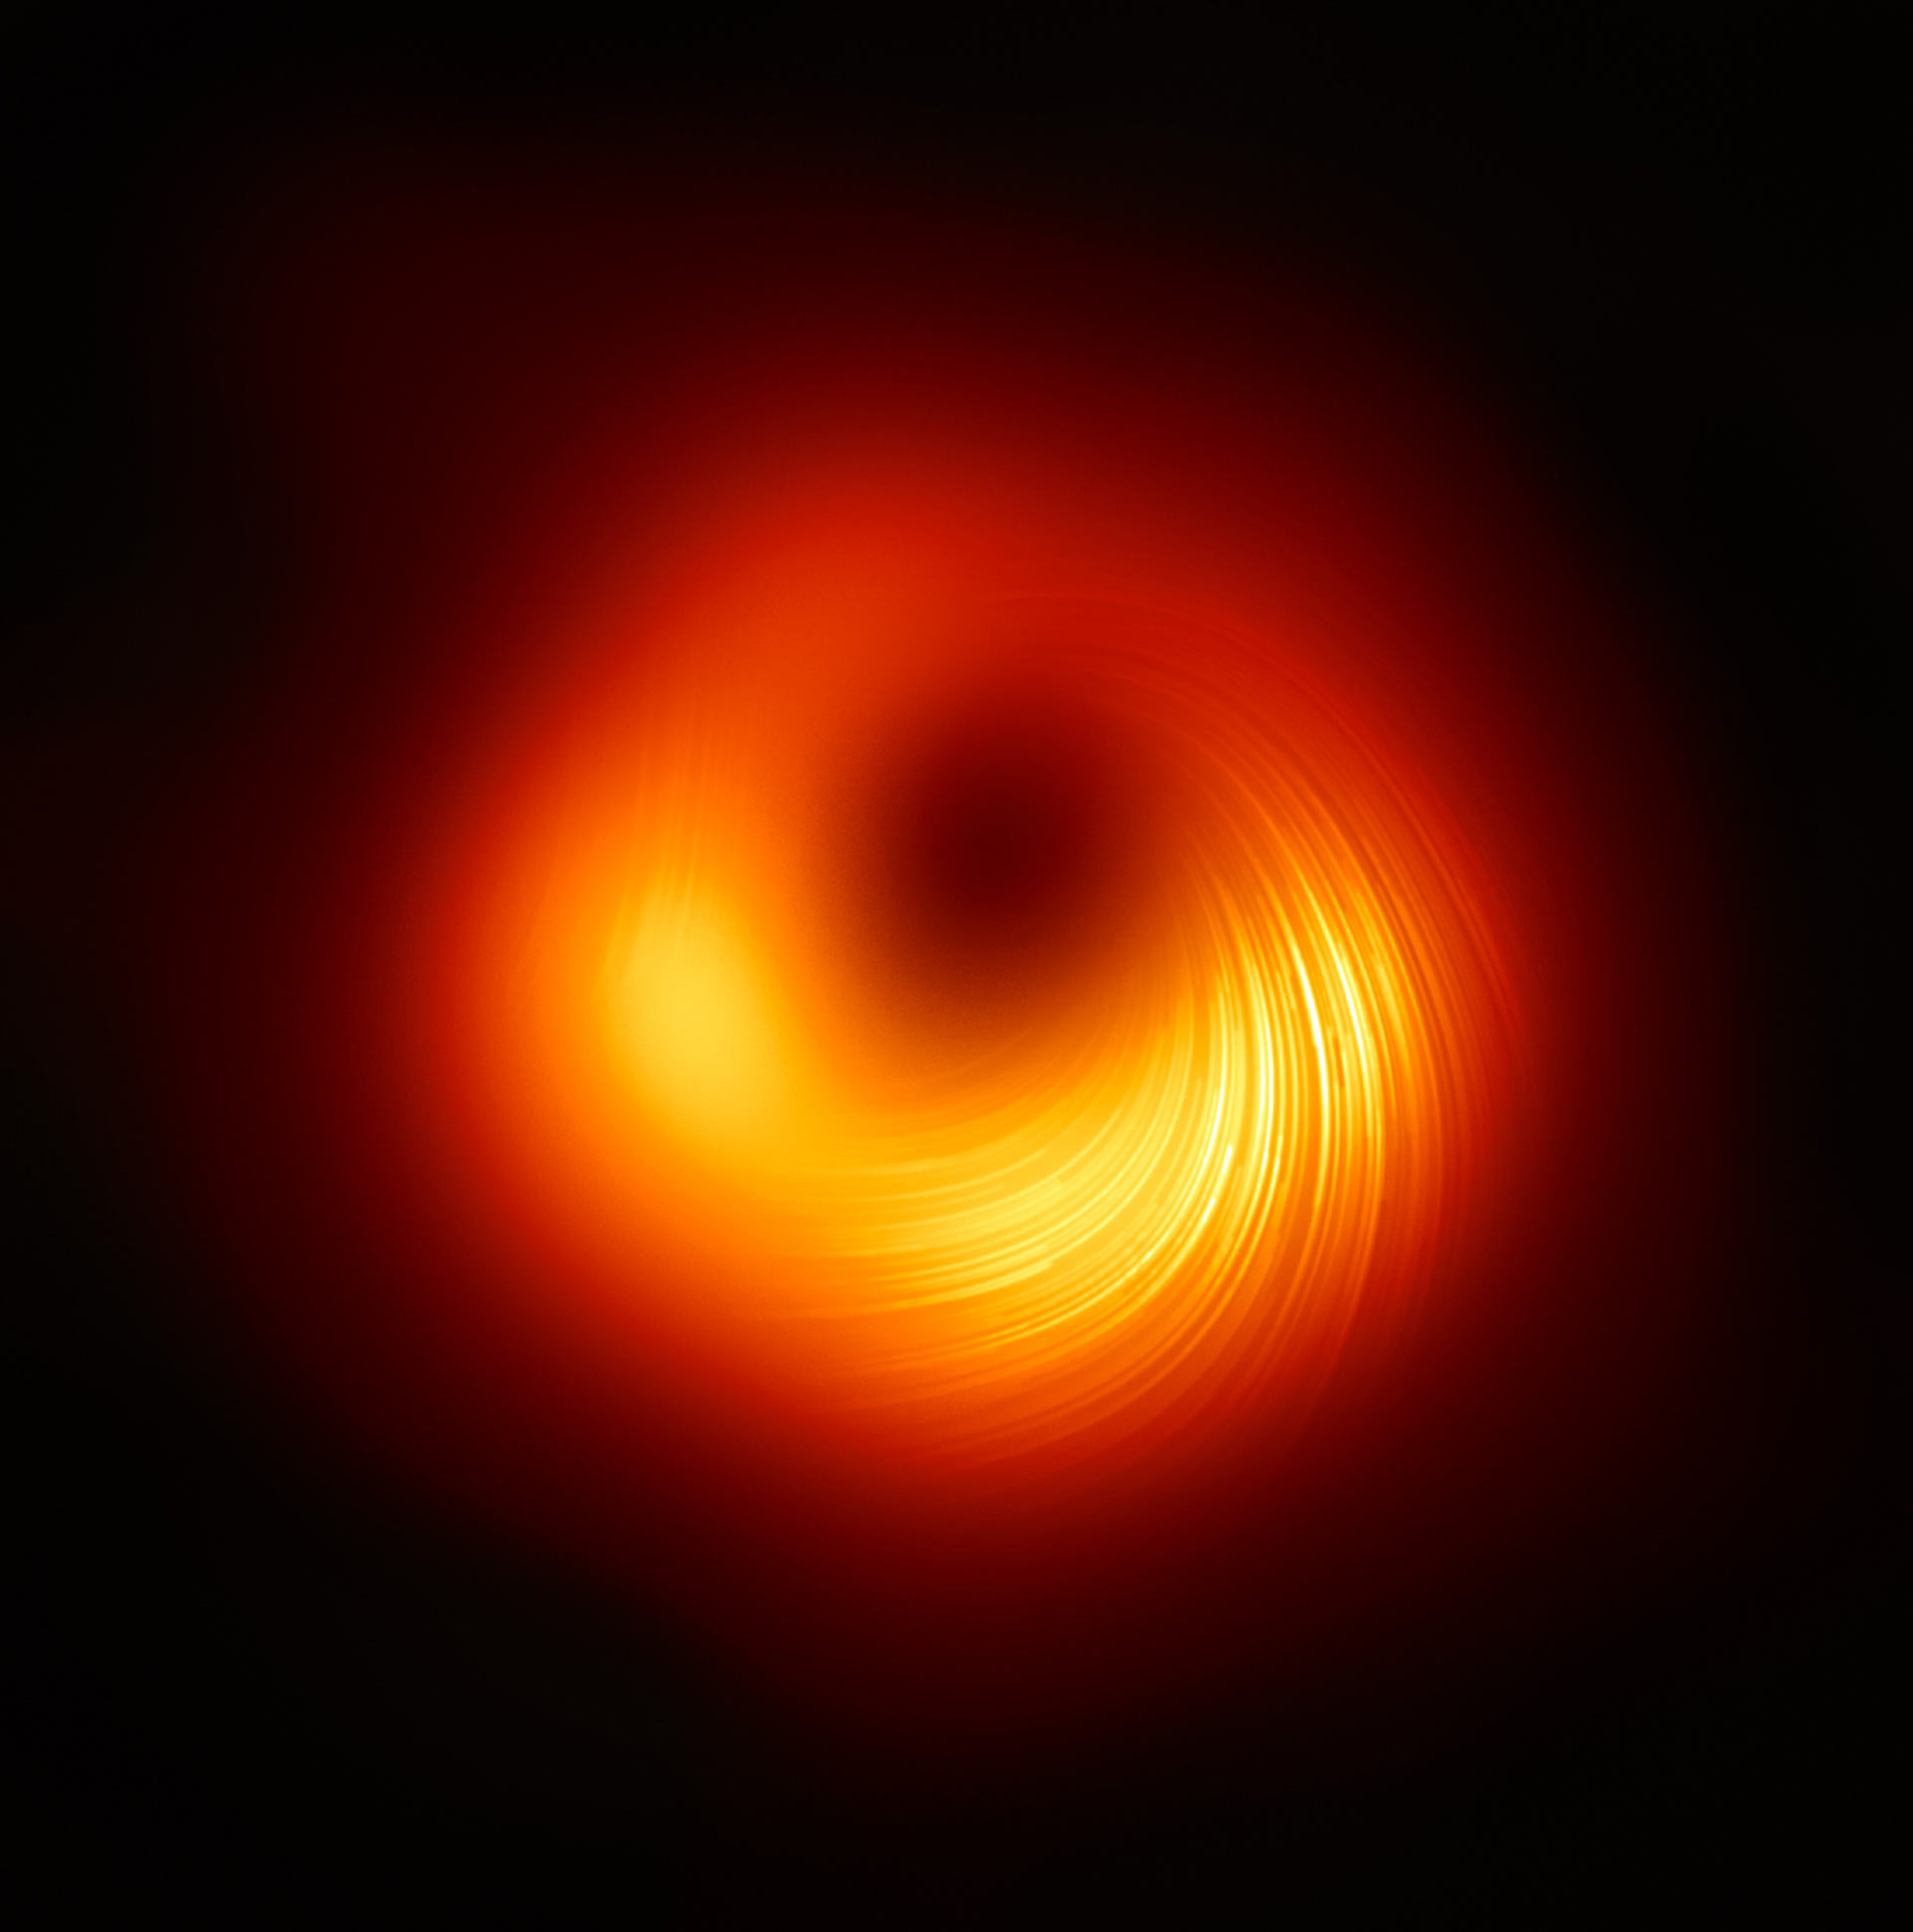
\includegraphics[width=0.5\textwidth]{bh.jpg}
\caption{Figura de agujero negro.}
\label{fig:agujero}
\end{figure}

\subsection{Nombre de la primera subsección}

hola pichula hola pichula hola pichula hola pichula hola pichula \textsc{hola pichula hola pichula hola pichula hola pichula hola pichula hola pichula hola pichula hola pichula hola pichula} hola pichula hola pichula hola pichula hola pichula hola pichula hola pichula hola pichula hola pichula hola pichula hola pichula hola pichula hola pichula hola pichula hola pichula hola pichula hola pichula hola pichula hola pichula hola pichula hola pichula ooo el agujero \ref{fig:agujero}

\begin{enumerate}
\item uno hola pichula hola pichula hola pichula hola pichula hola pichula hola pichula hola pichula hola pichula hola pichula hola pichula hola pichula hola pichula hola pichula hola pichula hola pichula hola pichula hola pichula hola pichula hola pichula hola pichula hola pichula hola pichula hola pichula hola pichula hola pichula hola pichula hola pichula hola pichula hola pichula hola pichula hola pichula hola pichula hola pichula hola pichula hola pichula hola pichula hola pichula hola pichula hola pichula

hola pichula hola pichula hola pichula hola pichula hola pichula hola pichula hola pichula hola pichula hola pichula hola pichula hola pichula hola pichula hola pichula hola pichula hola pichula hola pichula hola pichula hola pichula hola pichula hola pichula hola pichula hola pichula hola pichula hola pichula hola pichula hola pichula hola pichula hola pichula hola pichula hola pichula hola pichula hola pichula hola pichula hola pichula hola pichula hola pichula hola pichula hola pichula hola pichula \usespanishe{ahu61} \protect\citeA{ahu61}
\item dos hola pichula hola pichula hola pichula hola pichula hola pichula hola pichula hola pichula hola pichula hola pichula hola pichula hola pichula hola pichula hola pichula hola pichula hola pichula hola pichula hola pichula hola pichula hola pichula hola pichula hola pichula hola pichula hola pichula hola pichula hola pichula hola pichula hola pichula hola pichula hola pichula hola pichula hola pichula hola pichula hola pichula hola pichula hola pichula hola pichula hola pichula hola pichula hola pichula \cite{ahu61}
\begin{enumerate}
\item unouno
\item dosdos
\begin{enumerate}
\item solito
\item solito
\item solito
\item solito
\end{enumerate}
\end{enumerate}
\end{enumerate}

hola chao chao chao chao chao chao chao chao chao chao chao chao chao chao chao chao chao \citeA{ab94} chao \cite{ab94} chao chao chao chao chao chao chao chao chao chao chao chao chao chao chao chao chao chao chao chao chao chao chao chao chao chao chao chao chao chao chao chao chao chao chao chao chao chao chao chao chao chao chao chao chao chao chao chao chao chao chao chao chao chao chao chao chao chao chao chao chao chao chao chao chao chao chao chao chao chao chao chao chao chao chao chao chao chao chao chao chao chao chao chao chao chao chao chao chao chao chao chao chao chao chao chao chao chao chao chao chao chao chao chao chao chao chao chao chao $\mathbb{Hola como esta1s\Gamma\gamma\Lambda\omega\phi\Delta}⟁⅀ℽℼℾℿ$

\begin{itemize}
\item primero
\item segundo
\begin{itemize}
\item tercero
\item cuarto
\item quinto
\end{itemize}
\end{itemize}

\section{Nombre de la segunda sección}

hola hola chao

\subsection{Nombre de la primera subsección}

hola

\subsection{Nombre de la segunda subsección}

holis \(\mathbb{A}\)

\chapter{Nuevo capítulo}

\thispagestyle{fancy}

\begin{table}[h]
\centering
\begin{tabu}{ccc}
\hline\rowfont{\bfseries}
nombre & edad & ciudad \\
\hline
daniel & 22 & ancud \\
sofia & 21 & stgo \\
\hline
\end{tabu}
\caption{Una tabla.}
\label{tab:tab1}
\end{table}










\setcounter{chapter}{14}

\chapter{Increíble... ola que \emph{tal}}

\thispagestyle{fancy}



\finish{test}

\end{document}